\documentclass[aspectratio=169,11pt]{beamer}
\usetheme{default}
\usecolortheme{default}
\setbeamertemplate{navigation symbols}{}
\setbeamertemplate{footline}[frame number]
\definecolor{accent}{HTML}{1D4ED8}
\definecolor{muted}{HTML}{525252}
\setbeamercolor{structure}{fg=accent}
\setbeamercolor{frametitle}{fg=accent}
\setbeamerfont{frametitle}{series=\bfseries}
\usepackage{booktabs,tikz,xspace}
\usetikzlibrary{arrows.meta,positioning}
\RequirePackage{xspace}
% generated by review/scripts/make_numbers.py -- do not edit
\newcommand{\nOpenAlex}{515\xspace}
\newcommand{\nArxivRetrieved}{474\xspace}
\newcommand{\nArxivMatched}{48\xspace}
\newcommand{\nUsenixScanned}{1558\xspace}
\newcommand{\nUsenixMatched}{4\xspace}
\newcommand{\nIdentifiedDB}{567\xspace}
\newcommand{\nScreened}{504\xspace}
\newcommand{\nDuplicates}{63\xspace}
\newcommand{\nExcludedTA}{210\xspace}
\newcommand{\nExcludedTAECOne}{29\xspace}
\newcommand{\nExcludedTAECTwo}{112\xspace}
\newcommand{\nExcludedTAECThree}{4\xspace}
\newcommand{\nExcludedTAECFour}{34\xspace}
\newcommand{\nExcludedTAECFive}{31\xspace}
\newcommand{\nSoughtDB}{294\xspace}
\newcommand{\nNotRetrievedDB}{11\xspace}
\newcommand{\nAssessedDB}{283\xspace}
\newcommand{\nExcludedFTDB}{12\xspace}
\newcommand{\nExcludedFTDBECTwo}{6\xspace}
\newcommand{\nExcludedFTDBECThree}{1\xspace}
\newcommand{\nExcludedFTDBECFour}{3\xspace}
\newcommand{\nExcludedFTDBECFive}{2\xspace}
\newcommand{\nIncludedReportsDB}{271\xspace}
\newcommand{\nNotRetrievedOther}{4\xspace}
\newcommand{\nAssessedOther}{144\xspace}
\newcommand{\nExcludedFTOther}{19\xspace}
\newcommand{\nExcludedFTOtherECTwo}{2\xspace}
\newcommand{\nExcludedFTOtherECThree}{16\xspace}
\newcommand{\nExcludedFTOtherECFour}{1\xspace}
\newcommand{\nExcludedFTOtherECFive}{0\xspace}
\newcommand{\nIncludedReportsOther}{125\xspace}
\newcommand{\nForwardRetrieved}{446\xspace}
\newcommand{\nForwardNew}{275\xspace}
\newcommand{\nBackwardNew}{151\xspace}
\newcommand{\nReviewerKnown}{6\xspace}
\newcommand{\nUpdateRetrieved}{2140\xspace}
\newcommand{\nUpdateNew}{1460\xspace}
\newcommand{\nUpdateAuto}{997\xspace}
\newcommand{\nUpdateCandidates}{463\xspace}
\newcommand{\nUpdateSought}{68\xspace}
\newcommand{\nOtherScreened}{1886\xspace}
\newcommand{\nOtherExcludedTA}{1744\xspace}
\newcommand{\nSoughtOther}{148\xspace}
\newcommand{\nSoughtAll}{442\xspace}
\newcommand{\nIdentifiedTotal}{2459\xspace}
\newcommand{\nReportsIncluded}{396\xspace}
\newcommand{\nUpdateStudies}{61\xspace}
\newcommand{\nStudies}{362\xspace}
\newcommand{\nLinkedReports}{34\xspace}
\newcommand{\nFulltext}{90\xspace}
\newcommand{\nFulltextIncluded}{89\xspace}
\newcommand{\nSecondary}{88\xspace}
\newcommand{\nOriginIEEE}{232\xspace}
\newcommand{\nOriginACM}{26\xspace}
\newcommand{\nStudiesN}{362\xspace}
\newcommand{\nStudiesPreTwentyOne}{54\xspace}
\newcommand{\nStudiesSinceTwentyThree}{222\xspace}
\newcommand{\nPctSinceTwentyThree}{61\xspace}
\newcommand{\nYearMax}{2025\xspace}
\newcommand{\nYearMaxN}{59\xspace}
\newcommand{\nGroupInternetGeneric}{215\xspace}
\newcommand{\nGroupWirelessCellular}{56\xspace}
\newcommand{\nGroupSatelliteSpace}{22\xspace}
\newcommand{\nGroupIotAdHocSensor}{42\xspace}
\newcommand{\nGroupDataCenter}{27\xspace}
\newcommand{\nContribCtrl}{298\xspace}
\newcommand{\nContribMethod}{18\xspace}
\newcommand{\nContribAnalysis}{28\xspace}
\newcommand{\nContribFramework}{9\xspace}
\newcommand{\nContribDeploy}{9\xspace}
\newcommand{\nDesignN}{325\xspace}
\newcommand{\nFamTab}{25\xspace}
\newcommand{\nFamAc}{41\xspace}
\newcommand{\nFamNr}{129\xspace}
\newcommand{\nFamPg}{38\xspace}
\newcommand{\nFamIl}{10\xspace}
\newcommand{\nFamDqn}{36\xspace}
\newcommand{\nFamBandit}{9\xspace}
\newcommand{\nFamMarl}{28\xspace}
\newcommand{\nFamMo}{5\xspace}
\newcommand{\nFamLa}{1\xspace}
\newcommand{\nFamOff}{16\xspace}
\newcommand{\nFamHier}{3\xspace}
\newcommand{\nFamMeta}{7\xspace}
\newcommand{\nFamLlm}{2\xspace}
\newcommand{\nFamOther}{1\xspace}
\newcommand{\nFamKnownN}{196\xspace}
\newcommand{\nPctDeepKnown}{80\xspace}
\newcommand{\nPctTabularKnown}{13\xspace}
\newcommand{\nActParam}{30\xspace}
\newcommand{\nActCwnd}{90\xspace}
\newcommand{\nActAqm}{19\xspace}
\newcommand{\nActRate}{94\xspace}
\newcommand{\nActSelect}{10\xspace}
\newcommand{\nActBitrate}{32\xspace}
\newcommand{\nActOther}{8\xspace}
\newcommand{\nActBuffer}{10\xspace}
\newcommand{\nActMulti}{12\xspace}
\newcommand{\nActEcn}{10\xspace}
\newcommand{\nActSplit}{4\xspace}
\newcommand{\nActNr}{19\xspace}
\newcommand{\nHybrid}{93\xspace}
\newcommand{\nPctHybrid}{29\xspace}
\newcommand{\nPctHybridPre}{25\xspace}
\newcommand{\nPctHybridPost}{31\xspace}
\newcommand{\nCtrlSender}{222\xspace}
\newcommand{\nCtrlReceiver}{22\xspace}
\newcommand{\nCtrlNetwork}{62\xspace}
\newcommand{\nCtrlCentral}{19\xspace}
\newcommand{\nEmpiricalN}{358\xspace}
\newcommand{\nLevelSimulation}{144\xspace}
\newcommand{\nPctLevelSimulation}{40\xspace}
\newcommand{\nLevelEmulation}{45\xspace}
\newcommand{\nPctLevelEmulation}{13\xspace}
\newcommand{\nLevelRealnetwork}{57\xspace}
\newcommand{\nPctLevelRealnetwork}{16\xspace}
\newcommand{\nLevelNotreported}{112\xspace}
\newcommand{\nPctLevelNotreported}{31\xspace}
\newcommand{\nKnownLevelN}{246\xspace}
\newcommand{\nPctRealOfKnown}{23\xspace}
\newcommand{\nPctSimOnlyOfKnown}{59\xspace}
\newcommand{\nFTEmpiricalN}{80\xspace}
\newcommand{\nPctRealOfFT}{21\xspace}
\newcommand{\nCode}{38\xspace}
\newcommand{\nPctCode}{10\xspace}
\newcommand{\nCodeDesign}{25\xspace}
\newcommand{\nPctCodeDesign}{8\xspace}
\newcommand{\nGen}{35\xspace}
\newcommand{\nPctGen}{11\xspace}
\newcommand{\nFair}{63\xspace}
\newcommand{\nPctFair}{19\xspace}
\newcommand{\nDeploy}{9\xspace}
\newcommand{\nSrcFT}{81\xspace}
\newcommand{\nSrcAB}{278\xspace}
\newcommand{\nSrcKN}{3\xspace}
\newcommand{\nStateCoded}{148\xspace}
\newcommand{\nRewardCoded}{204\xspace}
\newcommand{\nToolMininet}{9\xspace}
\newcommand{\nToolPantheon}{6\xspace}
\newcommand{\nToolnsTwo}{5\xspace}
\newcommand{\nToolCustomsimulator}{14\xspace}
\newcommand{\nToolLoggeddataset}{18\xspace}
\newcommand{\nToolnsThree}{46\xspace}
\newcommand{\nToolRealnetwork}{6\xspace}
\newcommand{\nToolMahimahi}{7\xspace}
\newcommand{\nToolOMNeT}{6\xspace}
\newcommand{\nToolTestbed}{13\xspace}
\newcommand{\nToolOpenNetLab}{2\xspace}
\newcommand{\nStateSignalsN}{148\xspace}
\newcommand{\nStateCrossLayerRadio}{15\xspace}
\newcommand{\nStateQueueBufferInNetwork}{35\xspace}
\newcommand{\nStateThroughputDeliveryRate}{73\xspace}
\newcommand{\nStateApplicationSemantic}{14\xspace}
\newcommand{\nStateDelayRtt}{39\xspace}
\newcommand{\nStateLossDeliveryRatio}{27\xspace}
\newcommand{\nStateTelemetryNetworkSignals}{11\xspace}
\newcommand{\nStateWindowInFlight}{10\xspace}
\newcommand{\nStateEcnMarks}{4\xspace}
\newcommand{\nRewardFairness}{16\xspace}
\newcommand{\nRewardThroughput}{96\xspace}
\newcommand{\nRewardDelayLatency}{81\xspace}
\newcommand{\nRewardOther}{35\xspace}
\newcommand{\nRewardQoeApplication}{32\xspace}
\newcommand{\nRewardUtilityFunction}{20\xspace}
\newcommand{\nRewardEnergy}{5\xspace}
\newcommand{\nRewardLoss}{38\xspace}
\newcommand{\nRewardFlowCompletionTime}{8\xspace}
\newcommand{\nRewardPowerThrDelay}{5\xspace}
\newcommand{\nRewardMultiObjectiveVector}{7\xspace}
\newcommand{\nRewardFormalProperty}{1\xspace}
\newcommand{\nDesignFT}{67\xspace}
\newcommand{\nPracCodeOrArtifactReleasedAll}{25\xspace}
\newcommand{\nPracCodeOrArtifactReleasedFT}{17\xspace}
\newcommand{\nPracTestedOnConditionsOutsidAll}{35\xspace}
\newcommand{\nPracTestedOnConditionsOutsidFT}{13\xspace}
\newcommand{\nPracFairnessOrTcpFriendlinesAll}{63\xspace}
\newcommand{\nPracFairnessOrTcpFriendlinesFT}{25\xspace}
\newcommand{\nPracEvaluatedInEmulationOrOnAll}{87\xspace}
\newcommand{\nPracEvaluatedInEmulationOrOnFT}{29\xspace}
\newcommand{\nPracEvaluatedOnARealNetworkAll}{51\xspace}
\newcommand{\nPracEvaluatedOnARealNetworkFT}{15\xspace}
\newcommand{\nPracEvaluationEnvironmentNotAll}{108\xspace}
\newcommand{\nPracEvaluationEnvironmentNotFT}{4\xspace}
\newcommand{\nSetWan}{97\xspace}
\newcommand{\nSetGen}{118\xspace}
\newcommand{\nSetCell}{56\xspace}
\newcommand{\nSetSat}{22\xspace}
\newcommand{\nSetIot}{42\xspace}
\newcommand{\nSetDc}{27\xspace}
\newcommand{\nChInternetN}{215\xspace}
\newcommand{\nChInternetDesign}{184\xspace}
\newcommand{\nChInternetAnalysis}{31\xspace}
\newcommand{\nChInternetHybrid}{53\xspace}
\newcommand{\nChInternetPctHybrid}{29\xspace}
\newcommand{\nChInternetSim}{63\xspace}
\newcommand{\nChInternetPctSim}{34\xspace}
\newcommand{\nChInternetEmu}{27\xspace}
\newcommand{\nChInternetPctEmu}{15\xspace}
\newcommand{\nChInternetReal}{34\xspace}
\newcommand{\nChInternetPctReal}{18\xspace}
\newcommand{\nChInternetNR}{60\xspace}
\newcommand{\nChInternetPctNR}{33\xspace}
\newcommand{\nChInternetCode}{20\xspace}
\newcommand{\nChInternetGen}{25\xspace}
\newcommand{\nChInternetFair}{38\xspace}
\newcommand{\nChInternetSender}{132\xspace}
\newcommand{\nChInternetNetwork}{24\xspace}
\newcommand{\nChInternetCentral}{9\xspace}
\newcommand{\nChInternetActCwnd}{44\xspace}
\newcommand{\nChInternetActRate}{57\xspace}
\newcommand{\nChInternetActParam}{15\xspace}
\newcommand{\nChInternetActSelect}{7\xspace}
\newcommand{\nChInternetActBitrate}{29\xspace}
\newcommand{\nChInternetActEcn}{1\xspace}
\newcommand{\nChInternetActAqm}{16\xspace}
\newcommand{\nChInternetActBuffer}{2\xspace}
\newcommand{\nChInternetActSplit}{1\xspace}
\newcommand{\nChInternetFamKnown}{126\xspace}
\newcommand{\nChInternetMarl}{12\xspace}
\newcommand{\nChWirelessN}{120\xspace}
\newcommand{\nChWirelessDesign}{115\xspace}
\newcommand{\nChWirelessAnalysis}{5\xspace}
\newcommand{\nChWirelessHybrid}{25\xspace}
\newcommand{\nChWirelessPctHybrid}{22\xspace}
\newcommand{\nChWirelessSim}{55\xspace}
\newcommand{\nChWirelessPctSim}{48\xspace}
\newcommand{\nChWirelessEmu}{6\xspace}
\newcommand{\nChWirelessPctEmu}{5\xspace}
\newcommand{\nChWirelessReal}{12\xspace}
\newcommand{\nChWirelessPctReal}{10\xspace}
\newcommand{\nChWirelessNR}{42\xspace}
\newcommand{\nChWirelessPctNR}{37\xspace}
\newcommand{\nChWirelessCode}{4\xspace}
\newcommand{\nChWirelessGen}{6\xspace}
\newcommand{\nChWirelessFair}{22\xspace}
\newcommand{\nChWirelessSender}{76\xspace}
\newcommand{\nChWirelessNetwork}{28\xspace}
\newcommand{\nChWirelessCentral}{7\xspace}
\newcommand{\nChWirelessActCwnd}{44\xspace}
\newcommand{\nChWirelessActRate}{27\xspace}
\newcommand{\nChWirelessActParam}{12\xspace}
\newcommand{\nChWirelessActSelect}{2\xspace}
\newcommand{\nChWirelessActBitrate}{3\xspace}
\newcommand{\nChWirelessActEcn}{1\xspace}
\newcommand{\nChWirelessActAqm}{3\xspace}
\newcommand{\nChWirelessActBuffer}{7\xspace}
\newcommand{\nChWirelessActSplit}{3\xspace}
\newcommand{\nChWirelessFamKnown}{57\xspace}
\newcommand{\nChWirelessMarl}{9\xspace}
\newcommand{\nChDatacenterN}{27\xspace}
\newcommand{\nChDatacenterDesign}{26\xspace}
\newcommand{\nChDatacenterAnalysis}{1\xspace}
\newcommand{\nChDatacenterHybrid}{15\xspace}
\newcommand{\nChDatacenterPctHybrid}{58\xspace}
\newcommand{\nChDatacenterSim}{12\xspace}
\newcommand{\nChDatacenterPctSim}{46\xspace}
\newcommand{\nChDatacenterEmu}{3\xspace}
\newcommand{\nChDatacenterPctEmu}{12\xspace}
\newcommand{\nChDatacenterReal}{5\xspace}
\newcommand{\nChDatacenterPctReal}{19\xspace}
\newcommand{\nChDatacenterNR}{6\xspace}
\newcommand{\nChDatacenterPctNR}{23\xspace}
\newcommand{\nChDatacenterCode}{1\xspace}
\newcommand{\nChDatacenterGen}{4\xspace}
\newcommand{\nChDatacenterFair}{3\xspace}
\newcommand{\nChDatacenterSender}{14\xspace}
\newcommand{\nChDatacenterNetwork}{10\xspace}
\newcommand{\nChDatacenterCentral}{3\xspace}
\newcommand{\nChDatacenterActCwnd}{2\xspace}
\newcommand{\nChDatacenterActRate}{10\xspace}
\newcommand{\nChDatacenterActParam}{3\xspace}
\newcommand{\nChDatacenterActSelect}{1\xspace}
\newcommand{\nChDatacenterActBitrate}{0\xspace}
\newcommand{\nChDatacenterActEcn}{8\xspace}
\newcommand{\nChDatacenterActAqm}{0\xspace}
\newcommand{\nChDatacenterActBuffer}{1\xspace}
\newcommand{\nChDatacenterActSplit}{0\xspace}
\newcommand{\nChDatacenterFamKnown}{13\xspace}
\newcommand{\nChDatacenterMarl}{7\xspace}
\newcommand{\nTopicRTC}{43\xspace}
\newcommand{\nTopicMP}{21\xspace}
\newcommand{\nTopicQUIC}{13\xspace}
\newcommand{\nTopicSDN}{15\xspace}
\newcommand{\nTopicNDN}{5\xspace}
\newcommand{\nTopicNetSide}{39\xspace}
\newcommand{\nTopicAQM}{19\xspace}
\newcommand{\nTopicSelect}{10\xspace}
\newcommand{\nTopicParam}{31\xspace}
\newcommand{\nTopicAnalysis}{28\xspace}
\newcommand{\nTrainSim}{134\xspace}
\newcommand{\nTrainEmu}{36\xspace}
\newcommand{\nTrainTestbed}{13\xspace}
\newcommand{\nTrainReal}{6\xspace}
\newcommand{\nTrainData}{17\xspace}
\newcommand{\nTrainNR}{119\xspace}
\newcommand{\nTrainNsThree}{44\xspace}
\newcommand{\nPeriodAN}{36\xspace}
\newcommand{\nPeriodASim}{39\xspace}
\newcommand{\nPeriodAEmu}{17\xspace}
\newcommand{\nPeriodAReal}{17\xspace}
\newcommand{\nPeriodANR}{28\xspace}
\newcommand{\nPeriodBN}{53\xspace}
\newcommand{\nPeriodBSim}{38\xspace}
\newcommand{\nPeriodBEmu}{11\xspace}
\newcommand{\nPeriodBReal}{19\xspace}
\newcommand{\nPeriodBNR}{32\xspace}
\newcommand{\nPeriodCN}{101\xspace}
\newcommand{\nPeriodCSim}{39\xspace}
\newcommand{\nPeriodCEmu}{14\xspace}
\newcommand{\nPeriodCReal}{17\xspace}
\newcommand{\nPeriodCNR}{31\xspace}
\newcommand{\nPeriodDN}{168\xspace}
\newcommand{\nPeriodDSim}{42\xspace}
\newcommand{\nPeriodDEmu}{11\xspace}
\newcommand{\nPeriodDReal}{14\xspace}
\newcommand{\nPeriodDNR}{32\xspace}
\newcommand{\nScoreMedian}{1\xspace}
\newcommand{\nScoreMedianFT}{2\xspace}
\newcommand{\nScoreZero}{90\xspace}
\newcommand{\nPctScoreZero}{28\xspace}
\newcommand{\nScoreAtMostOne}{191\xspace}
\newcommand{\nPctScoreAtMostOne}{59\xspace}
\newcommand{\nScoreFourPlus}{12\xspace}
\newcommand{\nScoreFive}{1\xspace}
\newcommand{\nTrainReported}{206\xspace}
\newcommand{\nPctPracEnvReported}{67\xspace}
\newcommand{\nPctPracEmuReal}{27\xspace}

\xspaceaddexceptions{\%}
% generated by case_study/plot_case_study.py -- do not edit
\newcommand{\nCsNarrowRefUtil}{96\xspace}
\newcommand{\nCsNarrowRefQ}{0.03\xspace}
\newcommand{\nCsNarrowWorstUtil}{29\xspace}
\newcommand{\nCsNarrowJitterTenUtil}{29\xspace}
\newcommand{\nCsNarrowBwTwoHundredUtil}{63\xspace}
\newcommand{\nCsNarrowLossFiveUtil}{94\xspace}
\newcommand{\nCsNarrowVarQ}{0.71\xspace}
\newcommand{\nCsBroadRefUtil}{94\xspace}
\newcommand{\nCsBroadRefQ}{0.09\xspace}
\newcommand{\nCsBroadWorstUtil}{49\xspace}
\newcommand{\nCsBroadJitterTenUtil}{69\xspace}
\newcommand{\nCsBroadBwTwoHundredUtil}{69\xspace}
\newcommand{\nCsBroadLossFiveUtil}{93\xspace}
\newcommand{\nCsBroadVarQ}{0.48\xspace}
\newcommand{\nCsAimdRefUtil}{99\xspace}
\newcommand{\nCsAimdRefQ}{0.72\xspace}
\newcommand{\nCsAimdWorstUtil}{44\xspace}
\newcommand{\nCsAimdJitterTenUtil}{99\xspace}
\newcommand{\nCsAimdBwTwoHundredUtil}{87\xspace}
\newcommand{\nCsAimdLossFiveUtil}{44\xspace}
\newcommand{\nCsAimdVarQ}{1.78\xspace}
\newcommand{\nCsBbrRefUtil}{100\xspace}
\newcommand{\nCsBbrRefQ}{0.09\xspace}
\newcommand{\nCsBbrWorstUtil}{92\xspace}
\newcommand{\nCsBbrJitterTenUtil}{100\xspace}
\newcommand{\nCsBbrBwTwoHundredUtil}{95\xspace}
\newcommand{\nCsBbrLossFiveUtil}{95\xspace}
\newcommand{\nCsBbrVarQ}{1.76\xspace}
\newcommand{\nCsSeeds}{4\xspace}
\newcommand{\nCsSteps}{5\xspace}
\newcommand{\nCsTrainMinutes}{9\xspace}
\newcommand{\nCsCollapsed}{1\xspace}
\newcommand{\nCsCollapsedUtil}{3\xspace}

\graphicspath{{../survey/figures/}}
\newcommand{\RQ}[1]{\textbf{RQ#1}}

\title{Reinforcement Learning for Congestion Control}
\subtitle{A Systematic Survey of Designs, Evaluation Practice, and Barriers to Deployment}
\author{Gaurab Baral \and Nityashree Vangala}
\institute{CS 6043: Networking}
\date{Fall 2026}

\begin{document}

\begin{frame}
\titlepage
\end{frame}

% ------------------------------------------------------------------
\begin{frame}{Why learn congestion control?}
\begin{columns}[T]
\column{0.52\textwidth}
\begin{itemize}
  \item Classic CC (Reno, CUBIC, BBR, Copa, DCTCP) is \textbf{hand-tuned} for one kind of network.
  \item Wireless, satellite and data-center links break its assumptions: non-congestive loss, noisy delay, microsecond RTTs.
  \item RL: an agent watches throughput, delay and loss, adjusts the rate or window each interval, and is \textbf{rewarded} for high throughput and low delay.
  \item Aurora (2019) made deep RL the standard formulation, and the field has grown quickly since.
\end{itemize}
\column{0.46\textwidth}
\centering
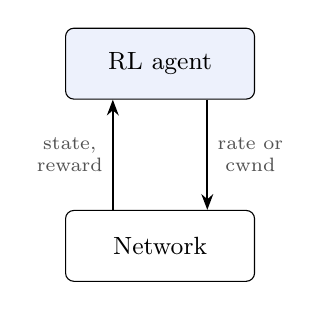
\begin{tikzpicture}[node distance=14mm, box/.style={draw, rounded corners=3pt, align=center, font=\small, minimum width=24mm, minimum height=9mm}, lab/.style={font=\scriptsize, align=center, text=muted}, >={Stealth[length=2mm]}]
  \node[box, fill=accent!8] (a) {RL agent};
  \node[box, below=of a] (n) {Network};
  \draw[->, thick] ([xshift=6mm]a.south) -- node[right, lab]{rate or\\ cwnd} ([xshift=6mm]n.north);
  \draw[->, thick] ([xshift=-6mm]n.north) -- node[left, lab]{state,\\ reward} ([xshift=-6mm]a.south);
\end{tikzpicture}
\end{columns}
\end{frame}

% ------------------------------------------------------------------
\begin{frame}{Research questions and method}
\begin{itemize}
  \item \RQ{1} \textbf{Design}: what do RL controllers observe, change, and learn from?
  \item \RQ{2} \textbf{Testing}: how are they trained and tested, and do they generalize?
  \item \RQ{3} \textbf{Deployment}: what stops operators from using them?
\end{itemize}
\vspace{4mm}
\textbf{PRISMA 2020 systematic review}, searches run 31 Oct 2026:
\begin{itemize}
  \item OpenAlex (stand-in for IEEE/ACM/Scopus), arXiv, USENIX NSDI/ATC, and forward and backward citation searching
  \item \nIdentifiedTotal{} records $\rightarrow$ \textbf{\nStudies{} studies} (\nReportsIncluded{} reports), 2016--2026
  \item Coded per study: setting, control point, state, action, reward, algorithm, training environment, \textbf{highest evaluation level}, out-of-distribution testing, fairness, code
  \item Everything is scripted and released: every decision, every number in the paper
\end{itemize}
\end{frame}

% ------------------------------------------------------------------
\begin{frame}{The field is growing fast}
\centering
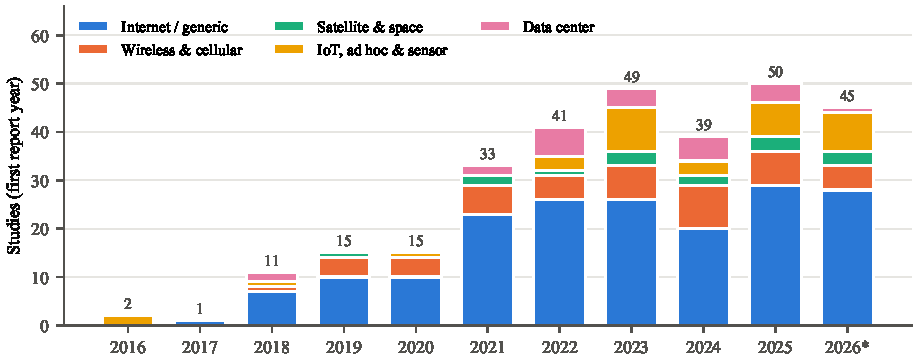
\includegraphics[width=0.86\textwidth]{fig_trend.pdf}\\[2mm]
\small \nPctSinceTwentyThree\% of studies appeared in 2023 or later. Settings: Internet/generic \nGroupInternetGeneric, wireless \nGroupWirelessCellular, IoT \nGroupIotAdHocSensor, data center \nGroupDataCenter, satellite \nGroupSatelliteSpace.
\end{frame}

% ------------------------------------------------------------------
\begin{frame}{\RQ{1}: What RL controllers observe, change and optimize}
\centering
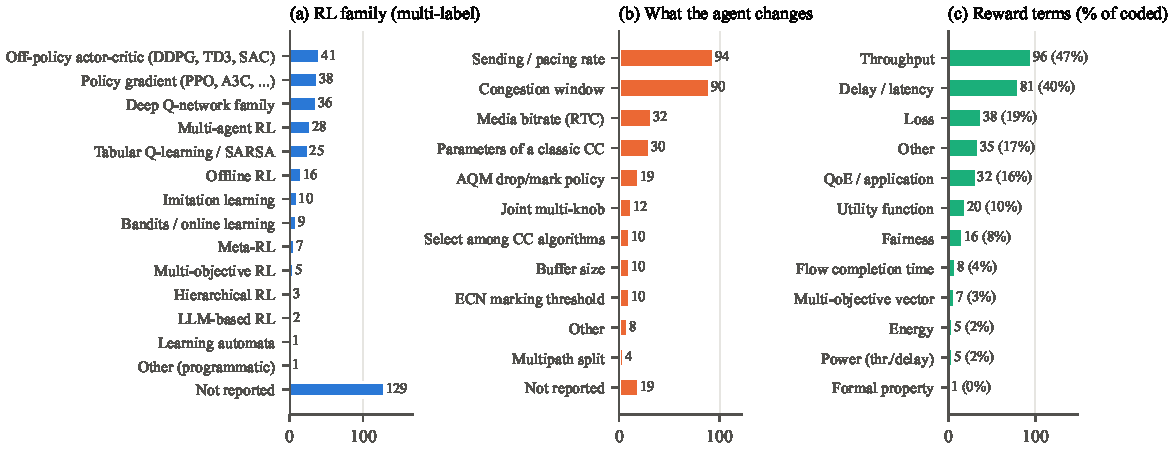
\includegraphics[width=\textwidth]{fig_design.pdf}\\[1mm]
\small Window (\nActCwnd) or rate (\nActRate) actions; throughput/delay/loss rewards. Only \nRewardFairness{} rewards include fairness.
\end{frame}

% ------------------------------------------------------------------
\begin{frame}{\RQ{1}: From clean-slate policies to hybrids}
\begin{columns}[T]
\column{0.5\textwidth}
\textbf{Clean slate} (2018--)
\begin{itemize}\small
  \item Aurora (PPO), Indigo (imitation), MVFST-RL (async.\ in QUIC)
  \item Many DQN/PPO/SAC variants evaluated in ns-3
\end{itemize}
\textbf{Hybrid}: learning tunes, selects or bounds classic CC
\begin{itemize}\small
  \item Orca: TD3 scales CUBIC's cwnd; Canopy adds certificates
  \item Spine, Libra, Mutant, Floo, TCP-RL
\end{itemize}
\column{0.5\textwidth}
\textbf{Learning from data}
\begin{itemize}\small
  \item Sage: offline RL from heuristics' logs
  \item RTC: offline-RL challenge on Teams logs
\end{itemize}
\vspace{3mm}
\begin{block}{Trend}
Hybrid share: \textbf{\nPctHybridPre\%} of designs before 2023 $\rightarrow$ \textbf{\nPctHybridPost\%} since.\\
Data centers: \nChDatacenterPctHybrid\% hybrid (ECN tuning per switch, e.g., ACC).
\end{block}
\end{columns}
\end{frame}

% ------------------------------------------------------------------
\begin{frame}{\RQ{2}: The evaluation ladder}
\begin{center}
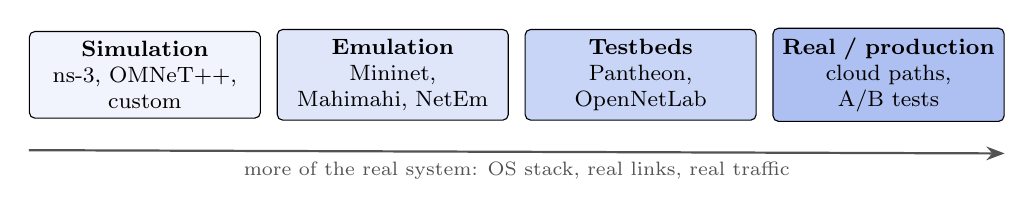
\begin{tikzpicture}[node distance=2mm, st/.style={draw, rounded corners=2pt, text width=27mm, minimum height=11mm, align=center, font=\footnotesize}]
  \node[st, fill=accent!6] (s) {\textbf{Simulation}\\ ns-3, \mbox{OMNeT++}, custom};
  \node[st, fill=accent!14, right=of s] (e) {\textbf{Emulation}\\ Mininet, Mahimahi, NetEm};
  \node[st, fill=accent!24, right=of e] (t) {\textbf{Testbeds}\\ Pantheon, OpenNetLab};
  \node[st, fill=accent!36, right=of t] (r) {\textbf{Real / production}\\ cloud paths, A/B tests};
  \draw[-{Stealth}, thick, muted] ([yshift=-4mm]s.south west) -- node[below, font=\scriptsize]{more of the real system: OS stack, real links, real traffic} ([yshift=-4mm]r.south east);
\end{tikzpicture}
\end{center}
\vspace{2mm}
\begin{alertblock}{Correction to our proposal}
\textbf{Wireshark is not a simulator.} It is a packet analyzer that captures and decodes real or emulated traffic. It is useful on every rung, but it does not model a network.
\end{alertblock}
\end{frame}

% ------------------------------------------------------------------
\begin{frame}{\RQ{2}: Where the evidence comes from}
\centering
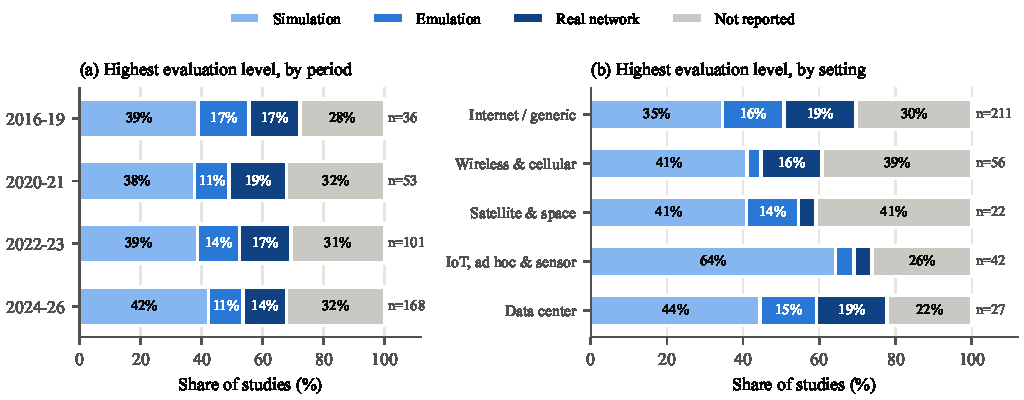
\includegraphics[width=0.92\textwidth]{fig_evaluation.pdf}\\[1mm]
\small Of studies with a known level, \textbf{\nPctSimOnlyOfKnown\%} are simulation-only and \textbf{\nPctRealOfKnown\%} reach a real network.\\
The real-network share \emph{fell}: \nPeriodBReal\% (2020--21) $\rightarrow$ \nPeriodDReal\% (2024--26).
\end{frame}

% ------------------------------------------------------------------
\begin{frame}{\RQ{2}: Practices that decide whether results transfer}
\centering
\small
\begin{tabular}{@{}lrrrr@{}}
\toprule
 & \multicolumn{2}{c}{All design studies} & \multicolumn{2}{c}{Full-text subset} \\
\cmidrule(lr){2-3}\cmidrule(l){4-5}
Practice & $n$ & \% of 266 & $n$ & \% of 64 \\
\midrule
Code or artifact released & 22 & 8 & 17 & 27 \\
Tested on conditions outside the training range & 30 & 11 & 13 & 20 \\
Fairness or TCP-friendliness evaluated & 54 & 20 & 24 & 38 \\
Evaluated in emulation or on a real network & 75 & 28 & 27 & 42 \\
Evaluated on a real network & 43 & 16 & 13 & 20 \\
Evaluation environment not reported & 86 & 32 & 4 & 6 \\
\bottomrule
\end{tabular}
\\[4mm]
\normalsize Independent re-evaluations: public RL controllers are \textbf{unfair in almost all setups} and lag under bandwidth or latency changes; a simulator-trained PPO reached \textbf{0.5\%} of a 10\,Gbit/s path.
\end{frame}

% ------------------------------------------------------------------
\begin{frame}{Case study: does the training distribution matter?}
\begin{columns}[T]
\column{0.42\textwidth}
\small
\begin{itemize}
  \item Aurora-style env: delayed feedback, latency features, multiplicative rate actions
  \item PPO, \nCsSeeds{} seeds $\times$ 2 training distributions:\\ \textbf{narrow} (1--5\,Mbit/s, no noise) vs.\ \textbf{broad} (1--100\,Mbit/s, loss, jitter, drift)
  \item Baselines: Reno-like AIMD, BBR-like
  \item One factor shifted at a time
\end{itemize}
\column{0.56\textwidth}
\centering
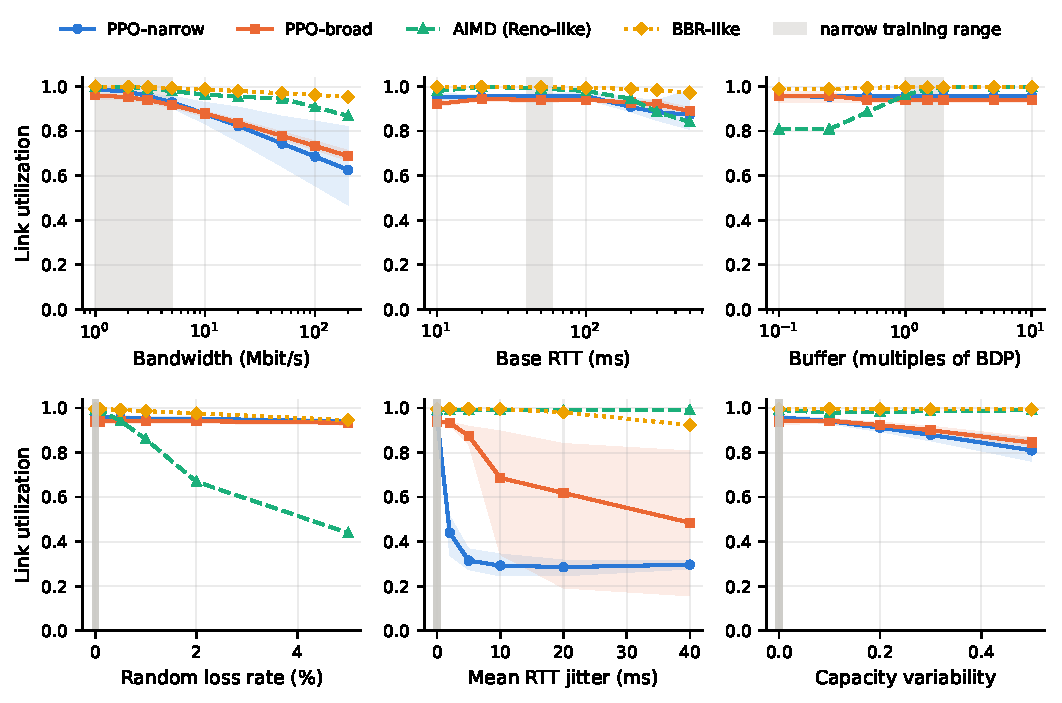
\includegraphics[width=\textwidth]{case_study_util.pdf}
\end{columns}
\end{frame}

% ------------------------------------------------------------------
\begin{frame}{Case study: results}
\centering
\resizebox{\textwidth}{!}{\begin{tabular}{@{}lrrrrrr@{}}
\toprule
 & \multicolumn{2}{c}{In distribution} & \multicolumn{4}{c}{Utilization (\%) under one shifted factor} \\
\cmidrule(lr){2-3}\cmidrule(l){4-7}
Controller & Util.\ (\%) & Queue (RTT) & 200\,Mbit/s & 5\% loss & 10\,ms jitter & Worst case \\
\midrule
PPO-narrow & 96 & 0.03 & 63 & 94 & 29 & 29 (20\,ms jitter) \\
PPO-broad & 94 & 0.09 & 69 & 93 & 69 & 49 (40\,ms jitter) \\
AIMD (Reno-like) & 99 & 0.72 & 87 & 44 & 99 & 44 (5\% loss) \\
BBR-like & 100 & 0.09 & 95 & 95 & 100 & 92 (40\,ms jitter) \\
\bottomrule
\end{tabular}
}
\vspace{4mm}
\begin{itemize}
  \item In distribution, the RL policy scores best on its own objective: \nCsNarrowRefUtil\% utilization with the smallest queue.
  \item 10\,ms of RTT jitter $\Rightarrow$ \textbf{\nCsNarrowJitterTenUtil\%}: latency features read noise as congestion.
  \item Broad training helps only within its coverage, queues more, and 1 of \nCsSeeds{} seeds collapsed.
  \item Learned and classic controllers fail \emph{differently}, so tests must target the policy's weaknesses.
\end{itemize}
\end{frame}

% ------------------------------------------------------------------
\begin{frame}{\RQ{3}: What deployed systems have in common}
\small
SmartIW/TCP-RL (search engine, $>$1 year), OnRL (543\,h, 151 users), Loki (101M sessions), ACC (production DCs), Floo, DuGu, Concerto, NVIDIA RL-CC (live NICs), Marten
\vspace{3mm}
\begin{enumerate}
  \item \textbf{The learned part is bounded}: 6 of 9 keep a classic algorithm or safeguard in the loop; the rest imitate logs or a solver, or are distilled into trees.
  \item \textbf{The operator owns the endpoints and the data}: it can A/B test, roll back, and train on its own logs.
  \item \textbf{The objective is narrow}: stalls, short-flow completion time, IOPS.
\end{enumerate}
\vspace{2mm}
No learned controller has been deployed for \emph{general} Internet traffic.
\end{frame}

% ------------------------------------------------------------------
\begin{frame}{\RQ{3}: Nine barriers}
\begin{columns}[T]
\column{0.5\textwidth}
\small
\begin{enumerate}
  \item Generalization under shift \hfill \emph{partly addressed}
  \item Safety, worst case \hfill \emph{runtime fallbacks}
  \item Fairness to CUBIC/BBR \hfill \emph{open}
  \item Overhead, datapath \hfill \emph{solved in principle}
  \item Interpretability \hfill \emph{prototypes}
\end{enumerate}
\column{0.5\textwidth}
\small
\begin{enumerate}\setcounter{enumi}{5}
  \item Adversarial robustness \hfill \emph{early}
  \item Objective specification \hfill \emph{active}
  \item Evaluation, reproducibility \hfill \emph{low adoption}
  \item Training cost, lifecycle \hfill \emph{open}
\end{enumerate}
\end{columns}
\vspace{5mm}
\small Only \nPctCodeDesign\% of design studies release code, and only \nPctGen\% test outside their training distribution.
\end{frame}

% ------------------------------------------------------------------
\begin{frame}{New direction: LLM-designed and LLM-driven controllers}
\small
\begin{itemize}
  \item \textbf{Designer} (offline): LLMs generate controller code or utility functions, scored in an emulator (PolicySmith, GenCC; He et al.: up to 27\% over BBR in a QUIC code base)
  \item \textbf{Translator}: natural-language intent $\rightarrow$ eBPF controller (NECC)
  \item \textbf{Policy} (online, triggered): CCA Reimagined, NetRL (+24\% utility vs.\ Orca), Trailblazer (Douyin A/B test)
\end{itemize}
\vspace{3mm}
\begin{block}{Assessment}
The hybrid lesson is being relearned: LLMs stay off the fast path. Generated \emph{code} is reviewable, which is good for trust. RL returns as the fine-tuning method. The evidence is still mostly emulation.
\end{block}
\end{frame}

% ------------------------------------------------------------------
\begin{frame}{Takeaways}
\begin{itemize}
  \item The bottleneck is not the learning algorithm but the \textbf{gap between training/test conditions and real networks}.
  \item Hybrids and learning from logs are how RL reached production.
  \item Agenda: distribution-shift benchmarks, harm-based coexistence tests, validated wireless and satellite emulators, runtime assurance, offline RL from logs, datapath co-design, LLMs at design time, lifecycle operations.
  \item Checklist: state the evaluation level, test out of distribution (including delay noise), compare with CUBIC/BBR, report seeds and failures, release code.
\end{itemize}
\vspace{4mm}
\centering\small Replication package: search scripts, all decisions, coded data, case study.
\end{frame}

\end{document}
